%% ID: angle_between_identical_masses
%% TITLE: Angle Between Two Identical Masses
%% TYPE: question
%% QUESTIONTYPE: scq
%% CONCEPTS: energy, momentum, momentumii, vectors
%% VIDEOS: 
%% LEVEL: 6
%% TOPIC: mechanics/dynamics
%% ORDER: 1

\begin{problem}[angle_between_identical_masses] 
{\exposition{A particle with mass \vari{m} travelling at speed  \vari{u} collides with a stationary particle of the same mass.} \question{What is the angle between the velocities of the two masses after this collision?}
\begin{enumerate}
	\item \choice[a]{\vari{26.6^{\circ}}}
	\item \choice[b]{\vari{45^{\circ}}}
	\item \choice[c]{\vari{53.2^{\circ}}}
	\item \choice[d]{\vari{90^{\circ}}}\correct
	\item \choice[e]{\vari{180^{\circ}}}
\end{enumerate}
}
{\stress{Another old question from multiple places}}
{\answer{The correct answer is (d).} By conservation of energy, \valuedef{\half mu^2}{\half mv_1^2 + \half mv_2^2}{}, where \vari{v_1} and \vari{v_2} are the speeds of the particles after the collision. In the zero momentum frame, both particles have a speed of \vari{\frac{u}{2}} in opposite directions, so on converting back into the lab frame, a triangle is created with sides of length \vari{u}, \vari{v_1} and  \vari{v_2}, with an angle \vari{\theta} between the final velocities of the two particles. Using the cosine rule, \valuedef{u^2}{v_1^2 +v_2^2 - 2 v_1 v_2 \cos \theta}{}. Combining this equation with that for conservation of energy gives \valuedef{2 v_1 v_2 \cos \theta}{0}, which is only possible if \valuedef{\cos \theta}{0}{}, so \valuedef{\theta}{90^{\circ}}{}

\begin{figure}[h]
	\centering
	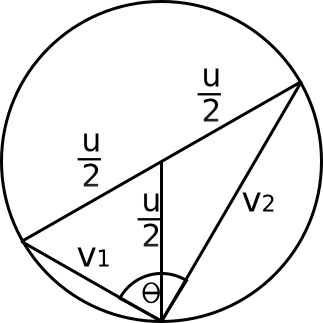
\includegraphics[width=0.5\textwidth]{../../../figures/dynamics_angle_between_identical_masses.svg}
	\caption{}\label{fig:Dynamics_angle_between_identical_masses}
\end{figure}
}
\end{problem}